%Wat zijn de sterke en zwakke punten van de controle-omgeving bij Seafood Connection?

\textbf{De controle-omgeving is de fundering van het interne betrouwbaarheidssysteem. Op dit element van de organisatie steunt de uitwerking van alle andere delen van het COSO-model.}

\medskip
\noindent
De aandachtspunten voor de uitwerking van de controle-omgeving tijdens dit onderzoek zijn: 

\begin{itemize}
    \item De cultuur binnen de organisatie;
    \item Het toezicht op de leiding;
    \item De houding ten opzichte van \gls{ic};
    \item Eventuele controleplichtigheid;
    \item De wet- en regelgeving binnen de branche;
    \item De economische omstandigheden binnen de branche.
\end{itemize}

De uitwerking van deze subdelen van het COSO-model moeten wel met elkaar overeenkomen. Wanneer de observeerbare cultuur drastisch verschilt tussen bijvoorbeeld de cultuur binnen de organisatie en de manier waarop de organisatorische maatregelen zijn ingericht, dan rijmt er iets niet met de 
\makebox[\textwidth][s]{verstrekte informatie voor de uitwerking van het onderzoek. Het is hierbij name-}

\begin{center}
  \makebox[\textwidth]{
\includegraphics[width=1.09\paperwidth]{img004}}
\end{center}

\noindent
lijk mogelijk dat de daadwerkelijke cultuur niet volledig in kaart is gebracht aangezien de cultuur als het ware dicteert hoe de organisatie in elkaar steekt. \citep{bivperspectief,bivpraktijk}


\bigskip
\noindent
Belangrijke elementen om nadere aandacht aan te besteden van de controle-omgeving van SCF, zijn: \\
\begin{itemize}
    \item Het al dan niet hebben van een code of conduct;
    \item Integriteit en ethische waarden;
    \item Voorbeeldgedrag van de leiding;
    \item Manier van leidinggeven;
    \item Wijze waarop de organisatie gestructureerd is;
    \item Delegatie van verantwoordelijkheden en bevoegdheden;
    \item Beleid op het gebied van personeelszorg.
\end{itemize}

Al de voorgenoemde elementen moeten samen komen tot één geheel waarin bondig kan worden samengevat hoe de cultuur in elkaar steekt. Dit wordt bewerkstelligd door de cultuur te typeren. Typering van de organisatie van Seafood Connection is mogelijk door gebruik te maken van het raamwerk van COSO. Er zijn een aantal principes uitgewerkt die voor elke deelvraag een beeld schetsen over wat voor soort organisatie SFC is, deze principes zijn te vinden in tabel \ref{tab:controleprincipes}.

\begin{table}[h]
    \centering
    \caption{Excerpt van de principes voor interne controle volgens COSO}
    \begin{tabular}{l l}
        \toprule
        \textbf{Element} & \textbf{Principe} \\
        \midrule
        Controleomgeving & 1. Tonen van een verbondenheid aan integriteit en \\
         & ethische waarden \\
         & 2. Vaststelling dat het bestuur toezicht op zich laat \\
         & uitoefenen en verantwoordelijk handelt \\
         & 3. Vaststellen van structuren, rapportagestromen, \\
         & autoriteiten, en verantwoordelijkheden \\
         & 4. Tonen van een verbondenheid aan het hebben \\
         & van competente werknemers \\
         & 5. Mensen verantwoordelijk houden \\
        \bottomrule
    \end{tabular}
    \label{tab:controleprincipes}
\end{table}

\begin{comment}
\begin{table}[!h]
    \centering
    \caption{Excerpt van de principes voor interne controle volgens COSO}
    \begin{tabular}{l l}
        \toprule
        \textbf{Element} & \textbf{Principe} \\
        \midrule
        Control environment & 1. Demonstrate commitment to integrity \\
         & and ethical values \\
         & 2. Ensure that board exercises oversight \\
         & responsibility \\
         & 3. Establish structures, reporting lines, \\
         & authorities and responsibilities \\
         & 4. Demonstrate commitment to a competent \\
         & workforce \\
         & 5. Hold people accountable \medskip \\
        Risk assessment & 6. Specify appropriate objectives \\
         & 7. Identify and analyze risks \\
         & 8. Evaluate fraud risks \\
         & 9. Identify and analyze changes that could \\
         & significantly affect internal controls \medskip \\
        Control activaties & 10. Select and develop control activities that \\
         & mitigate risks \\
         & 11. Select and develop technology controls \\
         & 12. Deploy control activities through policies \\
         & and procedures \medskip \\
        Information and communication & 13. Use relevant, quality information to \\
         & support the internal control function \\
         & 14. Communicate internal control information \\
         & internally \\
         & 15. Communicate internal control information \\
         & externally \medskip \\
        Monitoring activities & 16. Perform ongoing or periodic evaluations of \\
         & internal controls (or a combination of the two) \\
         & 17. Communicate internal control deficiencies \\
        \bottomrule
    \end{tabular}
    \label{tab:cosoprincipes}
\end{table}
\end{comment}

Vanuit het raamwerk van COSO zijn het eerste en derde principe typerend voor de organisatie van Seafood Connection. Dit blijkt uit de cultuur binnen de organisatie, het toezicht, de houding ten opzichte van interne controle, de geldende wet- en regelgeving, én de economische situatie waarin het bedrijf zich bevindt. 

\newpage 
\subsection{Cultuur}
Binnen Seafood Connection heerst een nuchtere en realistische manier van denken en een onaandoenlijke manier van werken richting de gestelde einddoelen. Dit uit zich doordat het hoofdkantoor van Seafood Connection haast volledig bestaat uit inwoners van voormalig eiland Urk. Hoewel normaal gesproken de herkomst van de werknemers er niet toe zal doen is dat hier wel het geval. Er heerst namelijk een sterke `klein dorp' mentaliteit waarin er ongeschreven sociale regels zijn en men snel aangesproken wordt op afwijkend gedrag ten opzichte van de groep. Seafood Connection is gehecht aan hard werken om op een eerlijke manier brood te verdienen. De onderneming werkt hard wat ook blijkt uit de slogan: \textit{``Alleen het beste is goed genoeg"}. \citep{sfcwebsite,quickscan} 

Een opvallend verschil met andere ondernemingen die op Urk gevestigd zijn is dat er een vaste en heldere organisatiestructuur is opgezet. Urker bedrijven kampen over het algemeen met een aantal zaken, namelijk:

\begin{enumerate}
    \item Moeite met opvolging en het doorgeven van kennis;
    \item Moeite met het meegaan in een veranderende wereld en inspelen op kansen;
    \item Moeite om een vaste organisatie op te zetten, waardoor veel bedrijven een familiecultuur of ad-hoc-cultuur hebben.
\end{enumerate}

Binnen de organisatie van Seafood Connection zijn vaste rapportagelijnen gelegd. Deze lijnen dienen er voor om alle neuzen dezelfde kant op te krijgen maar ook om het managementteam te voorzien van de nodige informatie om de onderneming aan te sturen. Iedereen bij Seafood Connection is goed geïnformeerd over het takenpakket en de af te leggen verantwoordelijkheden. Het management heeft een zekere voorbeeldfunctie, maar een ieder heeft een eigen functie en verantwoordelijkheid. Een zekere gelijkwaardigheid blijkt uit de afschaffing van een bonussysteem. Het beloningssysteem bestaat nu uit een vast salaris met riante sociale regelingen en zeer gunstige arbeidsvoorwaarden. Figuur \ref{fig:organogrampers} geeft de organisatie indeling weer, let ook op het onderscheid dat gemaakt is tussen de afdelingen. Deze figuur is ook te vinden in bijlage 3. Het organogram geeft een diep doordachte P-, G-, en M-indeling weer van de organisatie. \citep{quickscan}

\begin{figure}[!h]
    \centering
    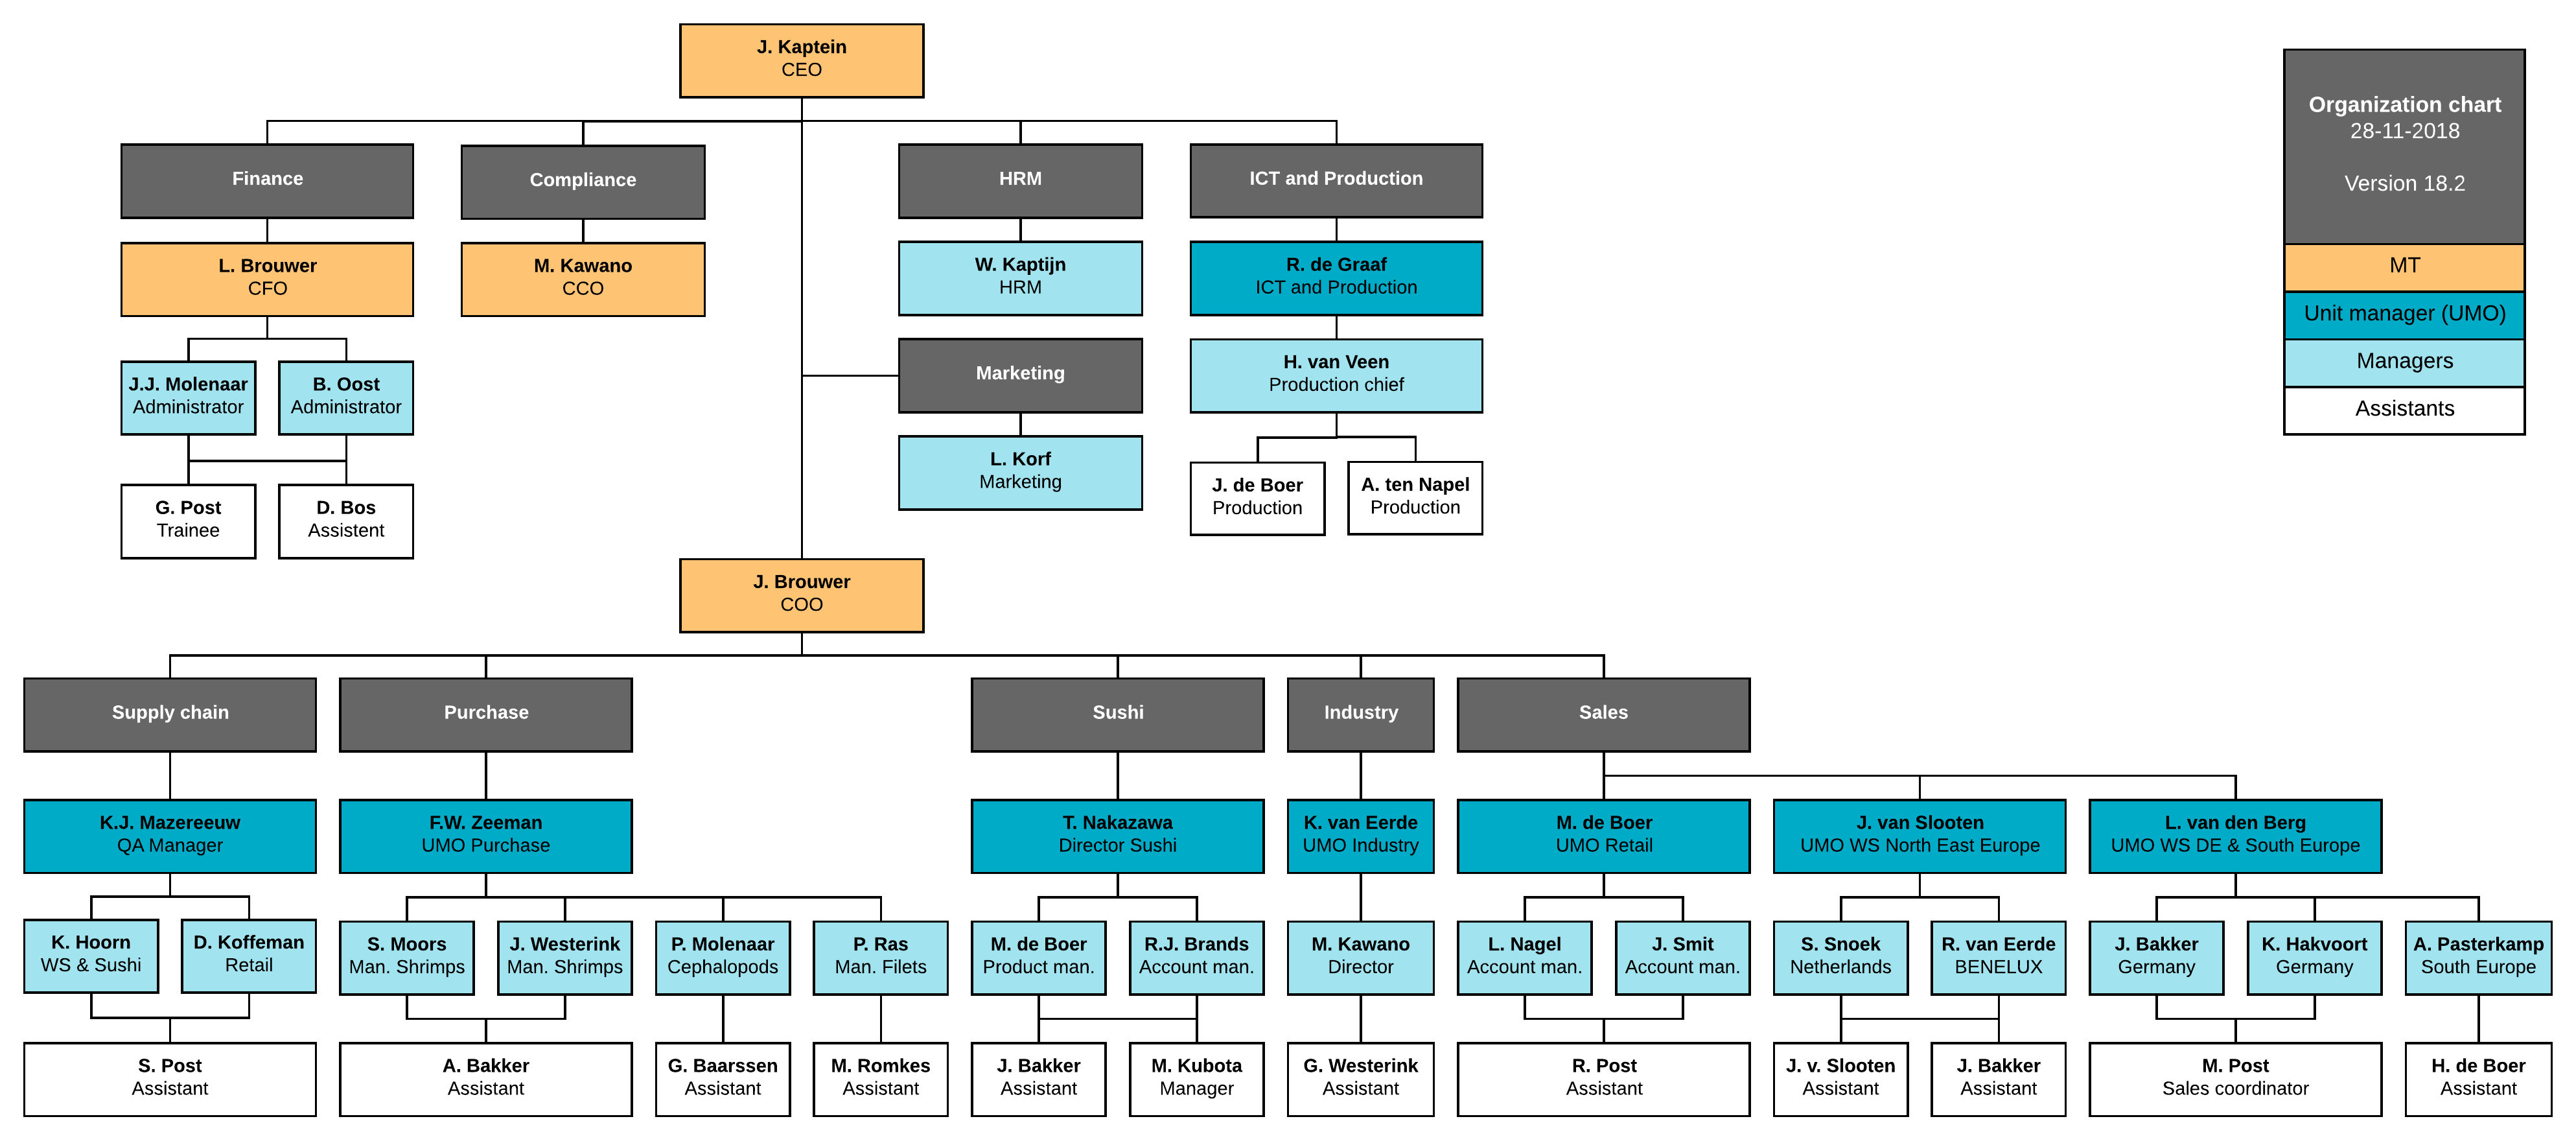
\includegraphics[width=1\textwidth]{organogrampersoneel}
    \caption{Organisatiestructuur SFC \citep{aoibsfc}}
    \label{fig:organogrampers}
\end{figure}

Naast het voorgaande hecht men veel waarde aan overleg. Frequente vergaderingen zijn belangrijk om niet alleen de plannen voor de komende periode te bespreken, maar ook om terug te kijken op voorgaande periode. De reflectie op de afgelopen periode dient als doel om zogenaamde \textit{forecasts} (begrotingen en cijfers voor de korte termijn) bij te stellen en beter aan te laten sluiten met de werkelijkheid. De inhoud en frequentie van de vergaderingen zijn weergegeven in figuur \ref{fig:overleg}.

\begin{figure}[!h]
    \centering
    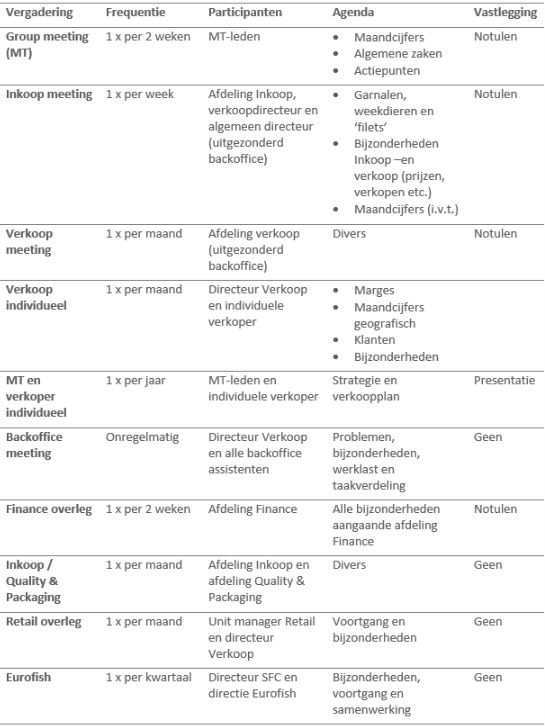
\includegraphics[width=1\textwidth]{overleg}
    \caption{Overlegstructuur SFC \citep{aoibsfc}}
    \label{fig:overleg}
\end{figure}

\newpage
\subsection{Toezicht}
Het Japanse moederbedrijf van SFC, Maruha Nichiro, oefent veel toezicht uit op SFC. Enkele werknemers van Maruha zijn werkzaam als expats binnen de organisatie. Ten tijde van schrijven zijn er drie expats werkzaam. Eén persoon die volledig gericht is op de compliance van SFC en in welke mate deze wordt nageleefd. Een ander bundelt allerlei financiële rapportagesets die opgestuurd worden naar Japan. Bij SFC is er een haast continue stroom van monitoring, het is de taak van de expat medewerker om deze informatie per kwartaal en per semester te vergaren en te verwerken op een manier die in overeenstemming is met de Japanse richtlijnen. Deze expat medewerker is ook een tussenschakel tussen de moeder en SFC. Alle vragen die de moeder heeft worden onderzocht door deze medewerker en afgestemd met het personeel van de Urker vestiging. \citep{aoibsfc}

Toezicht komt ook vanuit de hoek van de accountants. Er is een tussentijdse en eindejaarscontrole die de accountant uitvoert en waarvoor SFC werkt om een goedkeurende verklaring te kunnen krijgen. Vennootschappelijk en voor de doeleinden van dit onderzoek is Profinis de aanspreekbare accountant van SFC. Geconsolideerd is het internationale KPMG de controlerende accountant. \citep{quickscan}

Dit zijn de toezichthoudende partijen. Zoals uit figuur \ref{fig:organogram} blijkt is Maruha een grootaandeelhouder, maar ook Fishlink B.V. die volledig in handen is van CEO J. Kaptijn.

\begin{figure}[!h]
    \centering
    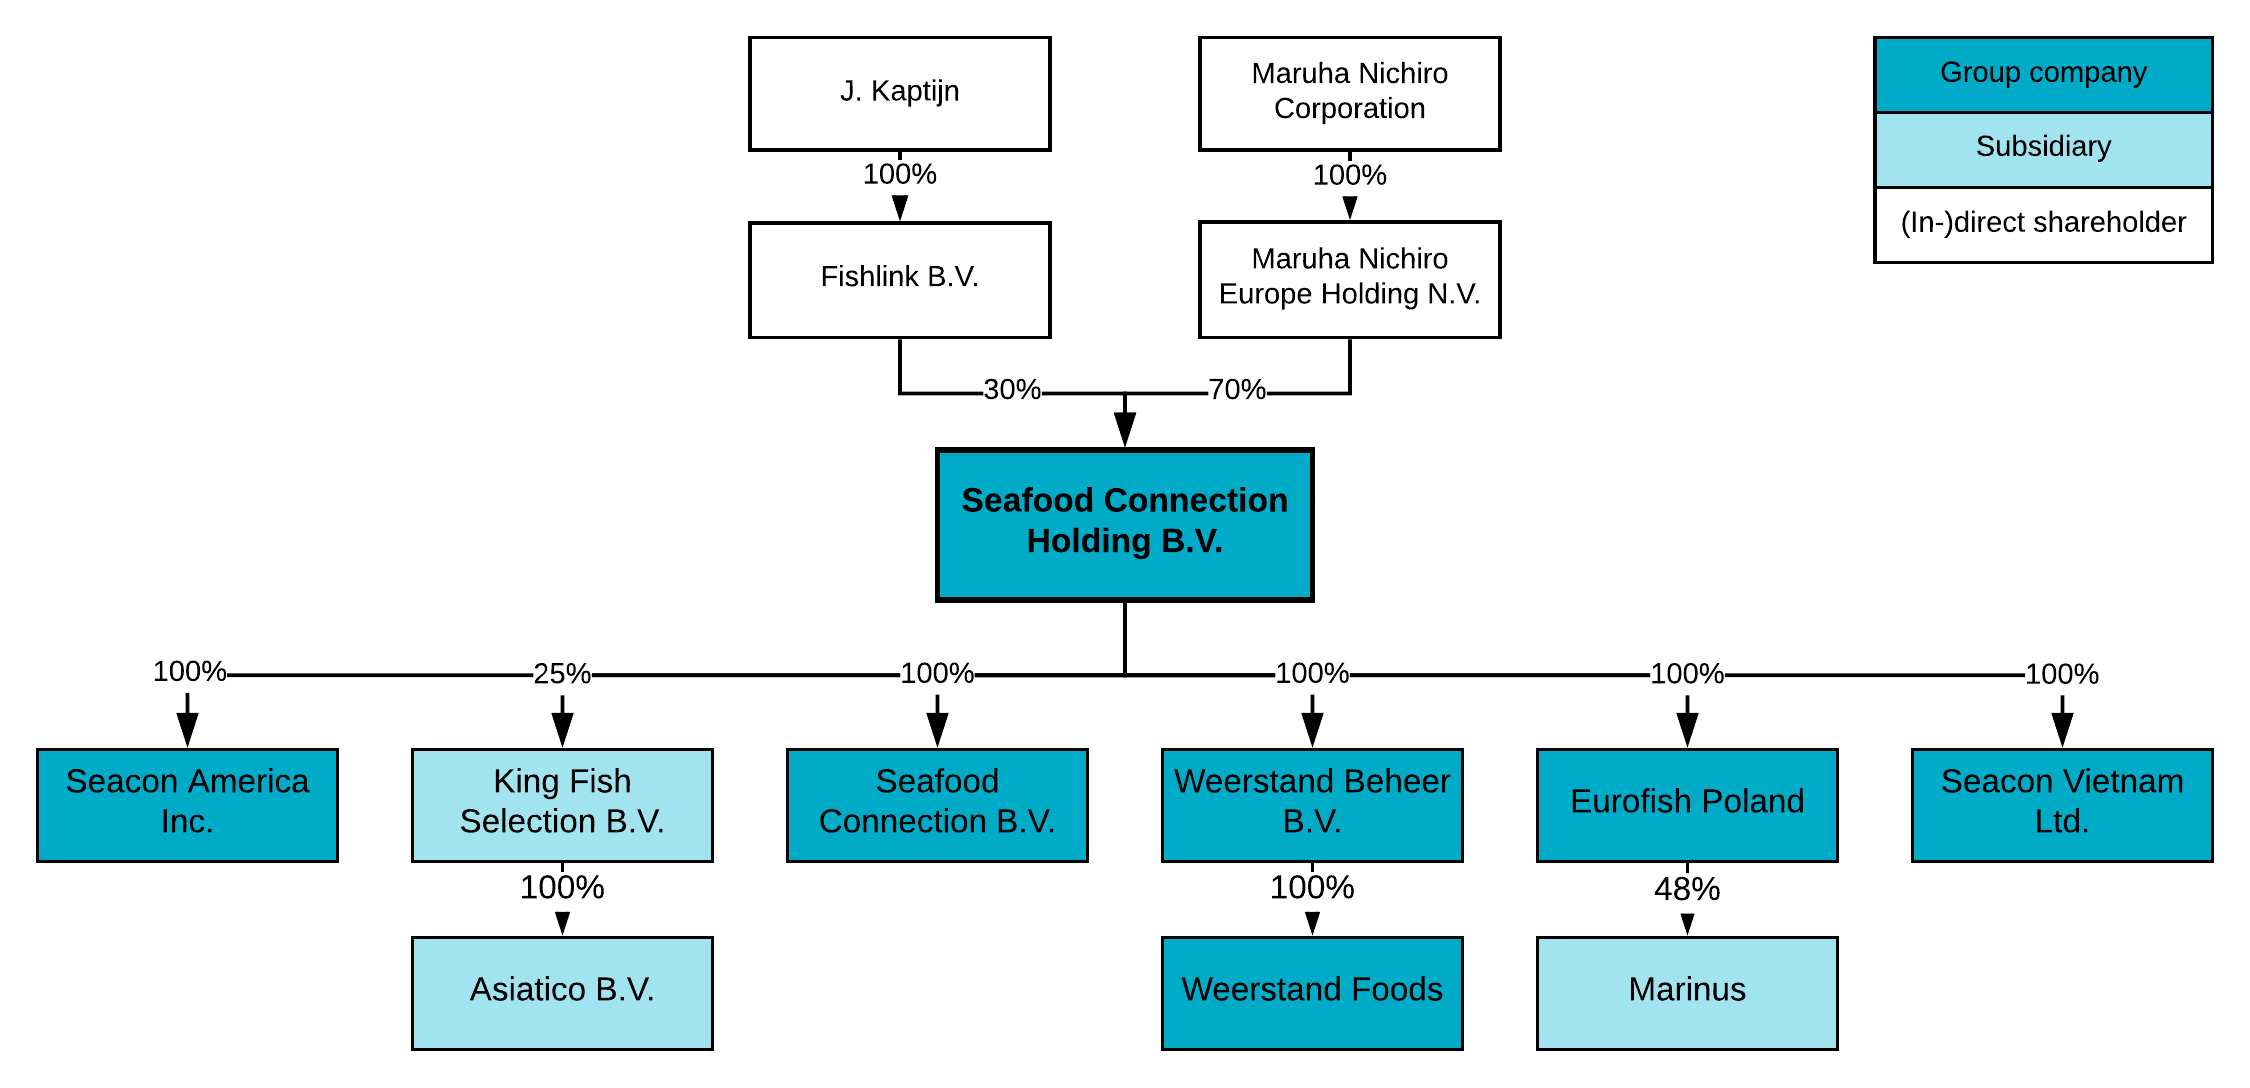
\includegraphics[width=1\textwidth]{organogram}
    \caption{Organogram SFC \citep{aoibsfc}}
    \label{fig:organogram}
\end{figure}


\subsection{Houding ten opzichte van \gls{ic}}
Seafood Connection maakt sterke groei mee de afgelopen jaren. Bij een groeiende onderneming hoort een groeiende organisatie. Hoe de verantwoordelijkheden en rapportagelijnen zijn vastgelegd verschilt per afdeling. Er wordt door het managementteam niet bewust gehouden aan formeel vastgelegde protocollen of maatregelen, wanneer nieuwe kansen te grijpen zijn worden deze met beide handen meteen aangepakt. Dit wil niet betekenen dat er tegen interne controle aangetrapt wordt, het tegendeel de interne controle hoort de bedrijfsvoering te versterken. Het management is van mening dat er niet een heel bureaucratisch proces moet worden doorlopen wanneer snel en onherroepelijk gehandeld moet worden. Het is niet het doel van de werkgever om de interne controle te gebruiken als leidraad voor de bedrijfsuitoefening, het is bedoeld als het afleggen van verantwoordelijkheid en het doen functioneren van de organisatie. Het management is tevreden met de vastgelegde interne controle. Er zijn geen goederen ongewild de onderneming verlaten en er is geen ernstig organisatorisch ontucht gebeurd. Hiermee is te stellen dat de huidige interne controle en de samenhangende controle omgeving werken. Er wordt kritisch nagedacht over het omgooien van interne controle en beheersing wanneer er een incident gebeurt dat gevolgen heeft voor de organisatie. Seafood Connection is wordt geleidt door gedreven ondernemers die kijken naar de toekomst, de interne controle speelt hierin de rol dat de organisatie aangepast wordt naar de wensen het management. \citep{quickscan}

\medskip
\subsection{Overige elementen van de controle omgeving}
Seafood Connection is onder de Dutch-GAAP controleplichtig in overeenstemming met artikel 396 BW2. Dit betekent concreet dat er strengere kwaliteitseisen zijn, extra informatie verschaft moet worden aan stakeholders, en dat wettelijke controle wordt uitgevoerd op het beleid, de organisatie en de financiële omgeving. Ook is Seafood Connection onderworpen aan nauwkeurig onderzoek vanuit de producten die geleverd worden. De EU heeft hoge normen voor voedsel en waren voor de import en export op een internationale markt. Seafood Connection heeft voor de verschillende producten allerlei keurmerken en certificaten. Dit is voor het onderzoek van mindere waarde en wordt hiermee alleen genoemd voor de beeldvorming.


\subsection*{Conclusie}
De controle omgeving is de fundering van de COSO piramide. Om deze reden omschrijft dit onderzoek met een brede blik naar alle elementen van de controle omgeving, maar wordt er minder aandacht aan de elementen die geen raakvlakken hebben met het functioneren van de primaire processen en het geldmiddelenbeheer. Bij het bespreken van de gevonden conclusies moet er worden bedacht dat al deze elementen een directe of indirecte invloed hebben op deze primaire processen tenzij anders aangegeven. 

\medskip
\noindent
\textit{De sterke punten van de controle omgeving:}
\begin{itemize}
    \item `Urker mentaliteit'. De medewerkers werken hard en op een ethisch verantwoorde manier;
    \item Problemen zijn goed bespreekbaar en gedrag afwijkend van de groep wordt snel aangesproken wat helpt om iedereen in lijn te brengen met de visie van het management;
    \item Het managementteam werkt onaandoenlijk richting de gestelde doelen en speelt in op kansen;
    \item In tegenstelling tot andere Urker bedrijven is de organisatie doordacht en helder ingericht. Er zijn vaste rapportagelijnen die duidelijk zijn voor iedereen, iedereen is bewust van zijn of haar takenpakket en verantwoordelijkheden;
    \item Het beloningssysteem behandeld iedereen gelijkwaardig door de afschaffing van bonussen. Riante sociale voorzieningen, loonschalen, en arbeidsvoorwaarden zorgen voor extra extrinsieke motivatie;
    \item Frequent overleg. Dit dient om te reflecteren op afgelopen perioden en vooruit te kijken naar de toekomst;
    \item Er is veel toezicht en interne controle door de aanwezigheid van afgevaardigden van het moederbedrijf;
    \item De bestaande interne controle, interne beheersing en bestuurlijke informatieverzorging werkt naar behoren. Er zijn geen incidenten geweest en er is geen sprake van ernstig ontucht.
\end{itemize}

\medskip
\noindent
\textit{De zwakke punten van de controle omgeving:}
\begin{itemize}
    \item Door het snelle handelen op nieuwe kansen is er vaak geen tijd of nut aan het doorlopen van een bureaucratisch proces;
    \item Er zijn relatief weinig stakeholders van het gevoerde beleid en de financiële omgeving, dit kan leiden tot zwakke interne controle;
    \item De onderneming groeit snel, de organisatie evolueert mee met deze groei. Het is nog de vraag of de behoeften van de organisatie goed aansluiten met de richting van de onderneming;
    \item Het managementteam is van mening dat interne controle volgt op de genomen beslissingen. Hoewel niet onterecht kan dit leiden dat er een kloof ontstaat tussen de formeel vastgelegde omgeving en de daadwerkelijke situatie;
    \item Interne controle wordt herzien op het moment dat er incidenten voordoen, er is geen organisatorisch anticiperende beleid.
\end{itemize}

\newpage